\chapter{Metodologia}
\label{chap:metodologia}

Para o desenvolvimento desse projeto, foi utilizado o ROS\textit{ Kinetic}, considerado uma das versões mais estáveis ROS. Ele é compatível apenas com o Ubuntu 16.04, tornando necessário a instalação do mesmo em \textit{dual boot}, mantendo o sistema operacional \textit{Windows} como segunda opção de \textit{boot}. Para isso, o tutorial utilizado para instalar o \textit{Ubuntu} em \textit{dual boot} no computador foi retirado do site \textit{Lcomlinux} \cite{ubuntu}. A Figura\ref{instacaoubuntu} mostra a página inicial de instalação do Ubuntu.

	\begin{figure}[H]
		\centering
		\Caption{{\label{instacaoubuntu}}Página inicial da instalação do Ubuntu}
		\UNIFORfig{}{
			\fbox{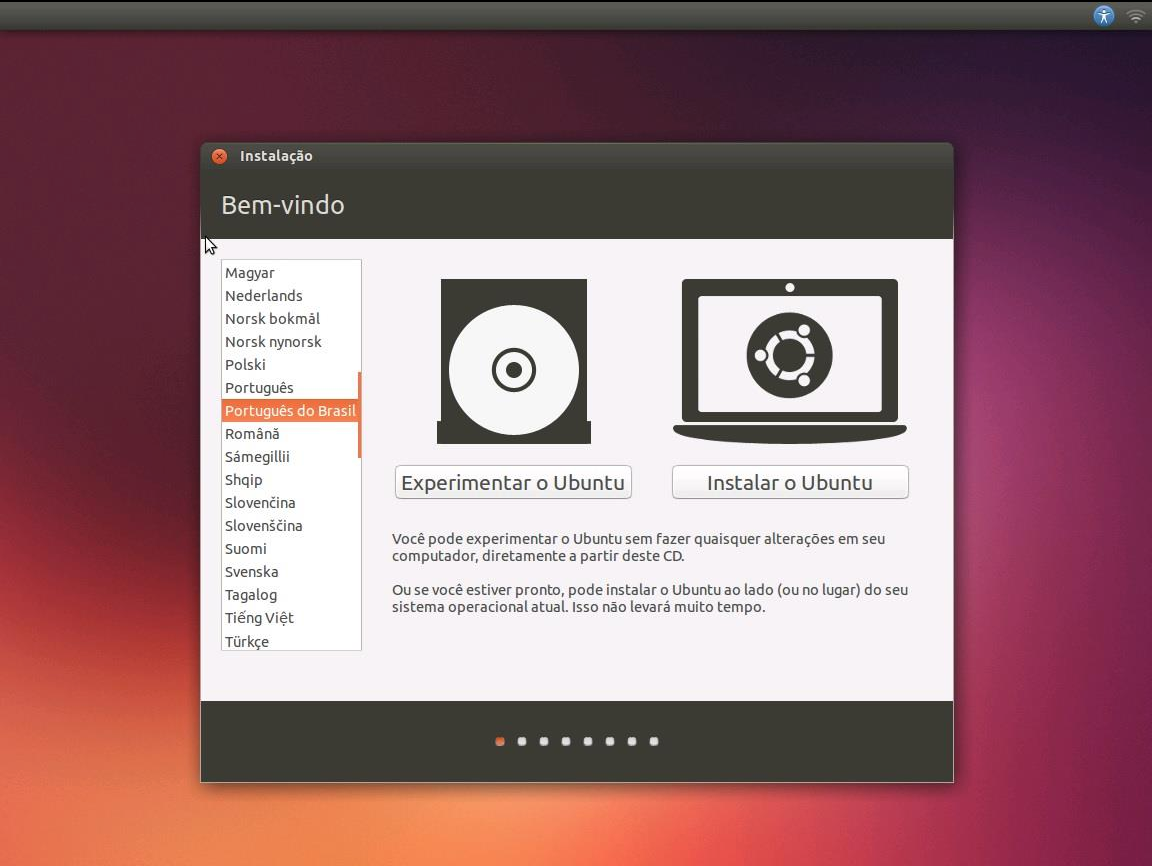
\includegraphics[width=14cm]{figuras/instalacaoubuntu.png}}
		}{
			\Fonte{Elaborado pelo autor}		}	
	\end{figure}
	
Após instalado o sistema, é preciso instalar o ROS e o \textit{python} 3.5 juntamente com os seus respectivos pacotes e biblioteca. O tutorial seguido para instalação do ROS foi retirado do própio site do Ros \cite{rosInstalacao}. Após a sua instalação e criação do seu \textit{Workspace} é preciso instalar os pacotes do Jaguar. Para isso, copie e cole a pasta \textit{DrRobotMotionSensorDriver-master} dentro da pasta src do \textit{Workspace} criada e novamente, no terminal aberto dentro do mesmo \textit{Workspace}, execute o comando catkin\_make. Faça a mesma coisa para a pasta \textit{drrobotV2\_player\-master}.

Caso não funcione, delete a pasta \textit{DrRobotMotionSensorDriver\-master}, mostrada na Figura\ref{arquivosROS} deixando somente o \textit{drrobotV2\_player\-master}, e copie os arquivos da pasta \textit{Drivers Ros/WorkSpace} e substitua os arquivos da sua pasta \textit{Devel} pelos arquivos da pasta fornecida e faça novamente o comando \textit{catkin\_make}. Antes de dar continuidade em qualquer comando no terminal para o ROS, execute o comando \textit{“source ...devel/setup.bash”} (substitua os três pontos pelo caminho do diretório do \textit{Workspace} do \textit{Ros}) depois faça o comando anterior. Normalmente é preciso executar o comando \textit{“source ...devel/setup.bash”} sempre que for executar algum \textit{node} do Jaguar. Esse comando não pode ser adicionado a inicialização do terminal pois ele é incompatível com a versão 3.5 do \textit{python}, tornando impossível a execução de programas \textit{python} dessa versão.

	\begin{figure}[H]
		\centering
		\Caption{\label{arquivosROS}Arquivos do \textit{Workspace} do ROS}
		\UNIFORfig{}{
			\fbox{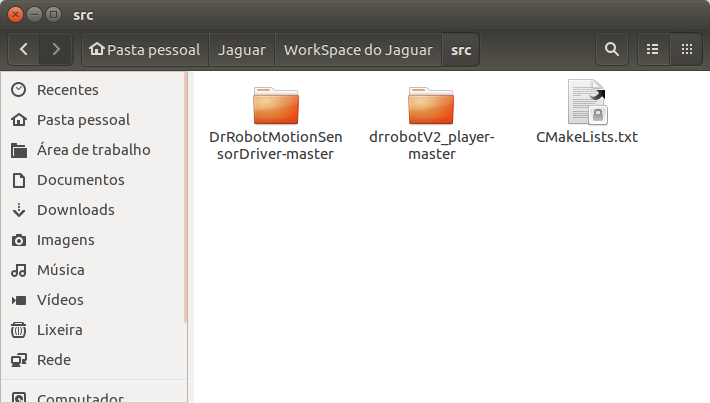
\includegraphics[width=14cm]{figuras/002.png}}
		}{
			\Fonte{Elaborado pelo autor}
		}	
	\end{figure}
	
Após feito a instalação do \textit{ROS} com os pacotes do Jaguar, é preciso instalar o \textit{python} 3.5 e suas bibliotecas para execução do programa. Para instalar o \textit{python} é muito simples: basta apenas executar os comandos abaixo. Eles instalam o \textit{python} 3.5 juntamente com o instalador de pacotes \textit{pip} de versão 2.7 e 3.5.
\begin{lstlisting}
sudo apt-get update
sudo apt-get install python3.5
sudo apt-get install python-pip 
sudo apt-get install python3-pip
\end{lstlisting}
Após a execução dos comandos o computador já deve estar com o \textit{python} e o \textit{pip} pronto para execução. Agora é preciso instalar as bibliotecas. Para o \textit{python} de versão 2.7, execute o seguinte comando no terminal dentro da pasta do projeto: 
\begin{lstlisting}
sudo pip install -r requerimentos2.7.txt
\end{lstlisting}
Para o \textit{python} de versão 3.5, execute o comando:
\begin{lstlisting}
sudo pip3 install -r requerimentos3.5.txt
\end{lstlisting}
Atualize o Ubuntu:
\begin{lstlisting}
sudo apt-get update
\end{lstlisting}
Para testar se todos os comandos foram executados corretamente, a sugestão é executar os arquivos \textit{savefile.py} e \textit{model.py} e verificar quais bibliotecas estão em falta. Para isso, abra o terminal dentro da pasta que se encontra esses dois arquivos e execute os seguintes comandos:
\begin{lstlisting}
Python3.5 savefile.py
\end{lstlisting}
Esse comando irá executar o arquivo \textit{savefile.py}. Se ele não executar, verifique quais bibliotecas estão em falta na janela do terminal. Faça a mesma coisa para o \textit{model.py}, executando o comando:
\begin{lstlisting}
Python model.py
\end{lstlisting}
Com todas as bibliotecas do \textit{python} funcionando, já é possível conectar o computador ao Jaguar. Use a senha 12345678 para conectar à rede “Jaguar”, mas antes modifique as configurações de IPv4 para os seguinte parâmetro:
\begin{lstlisting}
ip: 192.168.0.128
mascara de rede: 255.255.255.0
\end{lstlisting}
Após essa modificação é possível observar que o dispositivo já consegue conectar-se ao jaguar. 

\section{Ligando o ROS}
Para ligar o ROS siga os seguinte passos:

Abra o Terminal (Ctrl + Alt + T) e digite o comando:
\begin{lstlisting}
roscore
\end{lstlisting}
Esse comando irá executar o ROS ná máquina.

Abra outro terminal e execute:
\begin{lstlisting}
source (pasta do workspace)/devel/setup.bash
rosrun drrobot_jaguarV2_player drrobot_jaguarv2_player_node 
\end{lstlisting}
Há duas opções de comando do ROS para controlar o Jaguar: pelo teclado e pelo joystic

\subsection{Pelo teclado:}
Execute os comandos:
\begin{lstlisting}
source catkin_ws/devel/setup.bash
rosrun drrobot_jaguarV2_player drrobot_jaguarv2_keyboard_teleop_node
\end{lstlisting}

\subsection{Pelo joystick:}

Execute os comandos:
\begin{lstlisting}
source catkin_ws/devel/setup.bash
rosrun joy joy_node
\end{lstlisting}
Depois basta apenas plugar o Joystick no computador e controlar o Jaguar.

\section{programas essenciais}
\label{sec:programas essenciais}
Há quatro programas essenciais para o funcionamento do projeto: \textit{savefile.py, Model.py, Utils.py} e \textit{Drive.py}. Eles são todos programados em python e cada um desses arquivos desempenha uma função única e fundamental para o perfeito funcionamento do sistema autônomo no jaguar.

\subsection{\textit{Savefile.py}}
\label{sec:Savefile.py}

É o primeiro arquivo a ser executado. Ele foi criado pelo autor do projeto com o intuito de salvar as imagens capturadas pelo Jaguar e criar o arquivo \textit{driver\_log.csv} que contém a localização de cada uma das imagens juntamente com o ângulo de rotação e valor de aceleração do exato momento de captura da imagem. 


Esse arquivo deve ser executado enquanto o piloto controla o Jaguar para adquirir os dados de análise (no caso, o \textit{driver\_log.csv} e as imagens) e, de preferência, que seja obtido um grande número de dados para a criação de um bom modelo. 

\subsection{\textit{Model.py}}

É o arquivo de criação de modelo. 
Ele foi desenvolvido pelo a Udacity e adaptado para esse projeto com intuito de criar um modelo de predição para o Jaguar a partir do arquivo \textit{driver\_log.csv}. Nesse arquivo, é possível editar todos os parâmetros de entrada de dados e saída dos modelos. 

\subsection{\textit{Utils.py}}

 O jaguar consegue tirar fotos e gravar em alta resolução. Isso pode ser muito bom a princípio, porém imagens grandes podem aumentar ainda mais tempo de criação do modelo e predição. Então, para resolver esse problema a Udacity fornece o \textit{utils.py}: ele edita as imagens para facilitar o processamento do \textit{model.py} e \textit{drive.py}, já que o programa irá examinar \textit{pixel} por pixel de cada imagem, onde uma mudança em qualquer um dos \textit{pixels} o computador reconhece como uma nova imagem.

\subsection{\textit{Drive.py}}

Esse programa foi fornecido pelo Udacity e adaptado para esse projeto. Sua função é realizar o controle autônomo do Jaguar trabalhando em conjunto com os arquivos modelo (\textit{"model-002.h5"}, por exemplo) e o \textit{utils.py}. Ele recebe as imagens do Jaguar por ip e retorna comandos de velocidade e angulação para o \textit{Node} da rede do Jaguar. 

\section{Código}
\label{codigo}

\subsection{\textit{Savefile.py}}
\label{sec:Savefile.py}

	\begin{figure}[H]
		\centering
		\Caption{Linhas de código 1 à 10 do arquivo Savefile.py}
		\UNIFORfig{}{
			\fbox{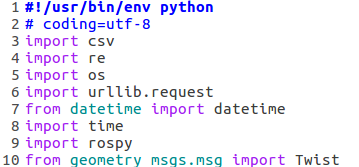
\includegraphics[width=8cm]{fig/1.png}}
		}{
			\Fonte{Elaborado pelo autor}
		}	
	\end{figure}
	
A primeira e segunda linha do código serve para utilizar caracteres especiais no código e comentários. As linhas seguintes (da 3 a 10) utilizam o método \textit{import} que serve para importar módulos para o código. Cada módulo será descrito abaixo:
\begin{description}
    \item[csv] linha 3. Serve para importar e exportar planilhas e bancos de dados;
    \item[re:] linha 4. Essa biblioteca serve para utilização de expressões regulares. Pode ser utilizado sequência de características unicode ou sequência de características 8 bits;
    \item[os:] linha 5. Serve para abrir, criar, ler e editar arquivos do sistema;
    \item[urllib.request:] linha 6. Um módulo de interface fácil para buscar dados em sites URL;
    \item[datetime:] linha 7. Manipula data e hora de forma simples ou complexa;
    \item[time:] linha 8. Função que recebe hora e data do sistema;
    \item[rospy:] linha 9. É uma biblioteca para \textit{python} que permite aos programadores terem acesso aos tópicos, serviços e parâmetros do \textit{ROS};
    \item[twist:] linha 10. Serve para enviar ou receber mensagens como pontos, vetores e valores comuns;
\end{description}

	\begin{figure}[H]
		\centering
		\Caption{Linhas de código 11 à 18 do arquivo Savefile.py}
		\UNIFORfig{}{
			\fbox{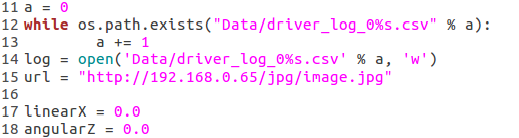
\includegraphics[width=12cm]{fig/2.png}}
		}{
			\Fonte{Elaborado pelo autor}
		}	
\end{figure}
	
Na linha 12, há um loop que procura o último driver\_log criado. Ele inicia com o valor '0', como é declarado na linha 11, e vai sendo incrementado até encontrar um valor de driver\_log que não tenha sido criado.
Na linha 15 é declarado o endereço das imagens retiradas pela câmera IP do Jaguar.

	\begin{figure}[H]
		\centering
		\Caption{Linhas de código 20 à 43 do arquivo Savefile.py}
		\UNIFORfig{}{
			\fbox{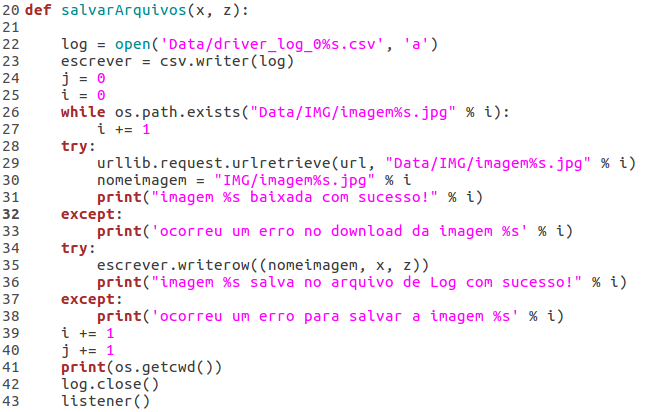
\includegraphics[width=15cm]{fig/3.png}}
		}{
			\Fonte{Elaborado pelo autor}
		}	
\end{figure}

O método salvarArquivos(), na linha 20, recebe como parâmetros a velocidade enviada para o Jaguar(variável x) e o ângulo (variável z). Primeiramente, na linha 22, será aberto o arquivo de \textit{driver\_logXX.csv} para poder escrever nele. Seguindo para a linha 26, o programa procura o valor da última imagem salva e usa um \textit{'try'} para tentar baixar a imagem fotografada pela câmera IP do Jaguar. Caso não funcione, ele exibe um erro na tela (erro nas linhas 33 e 38). 

Na linha 35 ele salva o nome da imagem, valor x e valor z dentro do arquivo csv e por último, na linha 43, ele chama o método \textit{listener()}.

	\begin{figure}[H]
		\centering
		\Caption{Linhas de código 53 à 66 do arquivo Savefile.py}
		\UNIFORfig{}{
			\fbox{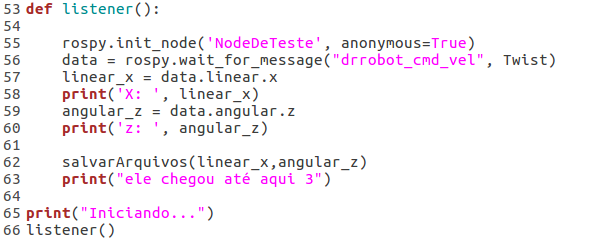
\includegraphics[width=15cm]{fig/5.png}}
		}{
			\Fonte{Elaborado pelo autor}
		}	
\end{figure}

O método \textit{listener()}, na linha 53, trata de criar um \textit{node} na rede do ROS para "ouvir" (nome utilizado para receber as mensagens de um determinado \textit{node} na rede do ROS) o \textit{node} \textit{ddrobot\_cmd\_vel} e atribuir os valores do data.linear.x e data.angular.z para o linear\_x e angular\_z, respectivamente.
Na linha 62 o método \textit{listener()} chama o método salvarArquivos() e atribui os valores de x e z aos valores linear\_x e angular\_z, respectivamente. E por último, já fora do método \textit{listener()}, esse mesmo método é chamado novamente, na linha 66, ao iniciar o programa.

\subsection{\textit{Model.py}}
\label{codigo_model}

	\begin{figure}[H]
		\centering
		\Caption{\label{model1}Linhas de código do 1 à 13 arquivo model.py}
		\UNIFORfig{}{
			\fbox{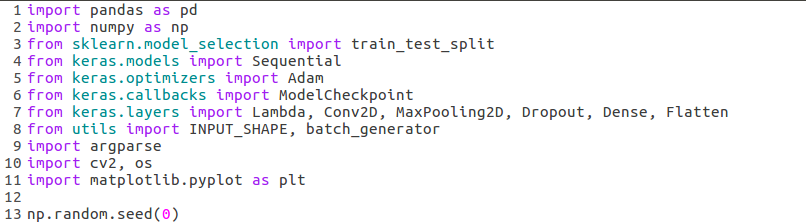
\includegraphics[width=16cm]{fig/10.png}}
		}{
			\Fonte{Elaborado pelo autor}
		}	
\end{figure}

Na Figura\ref{model1} são importadas as bibliotecas padrões que serão utilizadas no código \textit{model.py}, da linha 1 até a linha 11.

	\begin{figure}[H]
		\centering
		\Caption{\label{model2}Linhas de código do 16 à 34 arquivo model.py}
		\UNIFORfig{}{
			\fbox{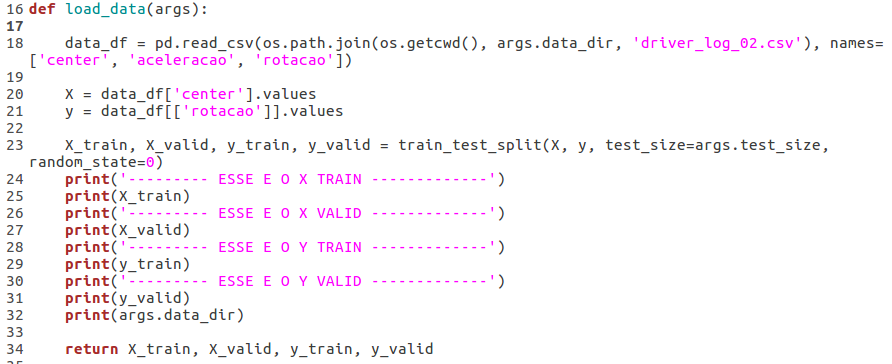
\includegraphics[width=16cm]{fig/11.png}}
		}{
			\Fonte{Elaborado pelo autor}
		}	
\end{figure}

Na linha 18 da Figura\ref{model2} a biblioteca \textit{pandas} é utilizada para abrir o arquivo \textit{.csv} criado pelo \textit{savefile.py} (\ref{sec:Savefile.py}) e transformá-lo em um \textit{dataframe} com coluna de nomes 'center', 'aceleracao' e 'rotacao'.
Na linha 20 e 21 os valores de 'center' e 'rotacao' são atribuídos as variáveis x e y, respectivamente. Na linha 23, o valor de X e y é divido em 80\% para treino (X\_train e x\_valid) e 20\% para teste (y\_train e y\_valid), no qual esse percentual está na variável test\_size.

	\begin{figure}[H]
		\centering
		\Caption{\label{model3}Linhas de código do 37 à 54 arquivo model.py}
		\UNIFORfig{}{
			\fbox{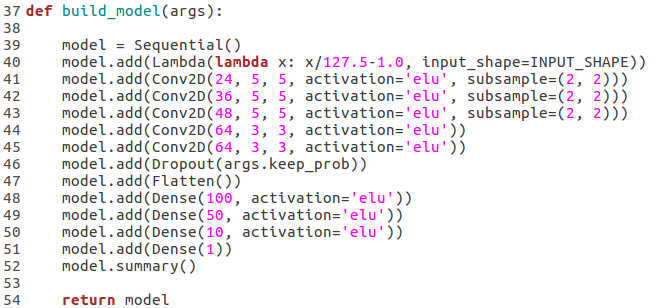
\includegraphics[width=16cm]{fig/12.png}}
		}{
			\Fonte{Elaborado pelo autor}
		}	
\end{figure}
A função da linha 37, \textit{build\_model(args)} cria a rede neural. Ela recebe como entrada um conjunto de argumentos que são declarados dentro do \textit{main()}.
Primeiramente é adicionado um espaço em branco na memória para o Keras trabalhar, na linha 39. 
Na linha 40, é adicionado uma camada de normalização de imagem. O número 127.5-1.0 foi escolhido pela comunidade de desenvolvedores depois de treinar com diferentes valores. Eles normalizam as imagens assim que são colocadas e evitam a saturação e fazem com que o gradiente funcione melhor. Ou seja, as imagens podem vim com sombras, de má qualidade. Essa função pode formatar e remodelar a imagem para trazer boas predições.
Nas linhas 40 à 45 são adicionadas 5 camadas convolucionais na rede neural. Ela recebe os seguintes argumentos: 

\begin{lstlisting}
conv2D(nb_filter, nb_row, nb_col, activation, subsample)
\end{lstlisting}

\begin{description}
    \item[nb\_filter:] Número de filtros de convolução a serem usados.
    \item[nb\_row:] Número de linhas no kernel da convolução.
    \item[nb\_col:] Número de colunas no kernel da convolução.
    \item[activation:] nome da função de ativação a ser usada. No caso, todas foram ELU:\textit{exponetial linear units}, usada para cuidar do problema gradiente de fuga
    \item[subsample:] tupla de comprimento 2. Fator pelo qual subamostra a saída.
    \item[Fonte:] \cite{kerasconv}
\end{description}
A camada de dropout, na linha 46, tem como função dar maior robustez à rede para previsões fora da amostra, buscando capturar informações populacionais ao invés de características amostrais. 
Dropout é um algoritmo relativamente novo para treinamento de redes neurais, que se fundamenta na eliminação aleatória de neurônios durante o processo de aprendizagem, para evitar a sobreadaptação aos dados (overfitting).

Na linha 47, o \textit{Flatten()} faz a preparação (achatamento) dos dados para trabalhar com series de camadas totalmente conectadas. As camadas convolucionais prepararam as imagens para serem tratadas pela rede neural. A intenção do código é achar uma relação das imagens com o \textit{steering\_angle} e o \textit{throttle}.

Da linha 48 até a linha 51 é criada a rede neural totalmente conectada. É possível observar que número de neurônios dessa rede vai reduzindo conforme a adesão de novas camadas, até chegar a um neurônio, na linha 51. 

Na linha 51 há uma função para imprimir os valores dos \textit{layers} e na 54 a função retorna o modelo criado.

	\begin{figure}[H]
		\centering
		\Caption{\label{model4}Linhas de código do 57 à 74 arquivo model.py}
		\UNIFORfig{}{
			\fbox{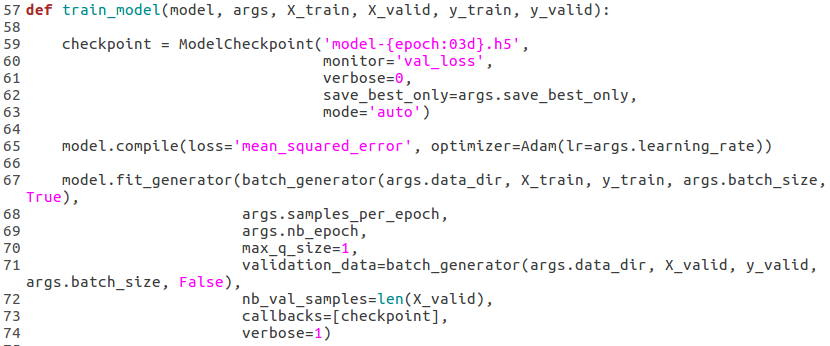
\includegraphics[width=16cm]{fig/13.png}}
		}{
			\Fonte{Elaborado pelo autor}
		}	
\end{figure}

A função \textit{train\_model()}, linha 57 da Figura\ref{model4}, tem como função treinar o modelo criado. Na linha 59, há um método que salva um modelo a cada \textit{epoch} (quantidade de vezes que o conjunto será treinado), caso ele tenha um \textit{'val\_loss'} menor que o anterior.

O Compilador do modelo, na linha 65, utiliza o método \textit{'mean\_squared\_error'}, que calcula a diferença entre o quadrado do valor esperado e o quadrado do valor obtido e tira a média de todos os valores obtidos para achar o erro. Esse método utiliza o otimizador Adam, que é um gradiente de descida.

\[\sum_{1}^{n}\frac{(valor\_real - valor\_obtido)^{2}}{n}\]

Na linha 67, o \textit{mode.fit\_generator} faz o treinamento do modelo. Ele utiliza o método \textit{batch\_generator()} do arquivo \textit{utils.py} e argumentos do \textit{main()} para fazer o treinamento e o \textit{checkpoint} da linha 59 para salvar o modelo treinado.

	\begin{figure}[H]
		\centering
		\Caption{\label{model5}Linhas de código do 77 à 80 arquivo model.py}
		\UNIFORfig{}{
			\fbox{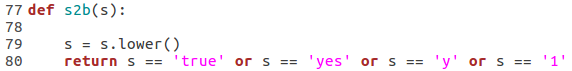
\includegraphics[width=14cm]{fig/14.png}}
		}{
			\Fonte{Elaborado pelo autor}
		}	
\end{figure}

O método \textit{s2b(s)} da Figura\ref{model5} é um simples método utilizado no \textit{main()} para converter \textit{strings} em valores booleanos.

	\begin{figure}[H]
		\centering
		\Caption{\label{model6}Linhas de código do 83 à 108 arquivo model.py}
		\UNIFORfig{}{
			\fbox{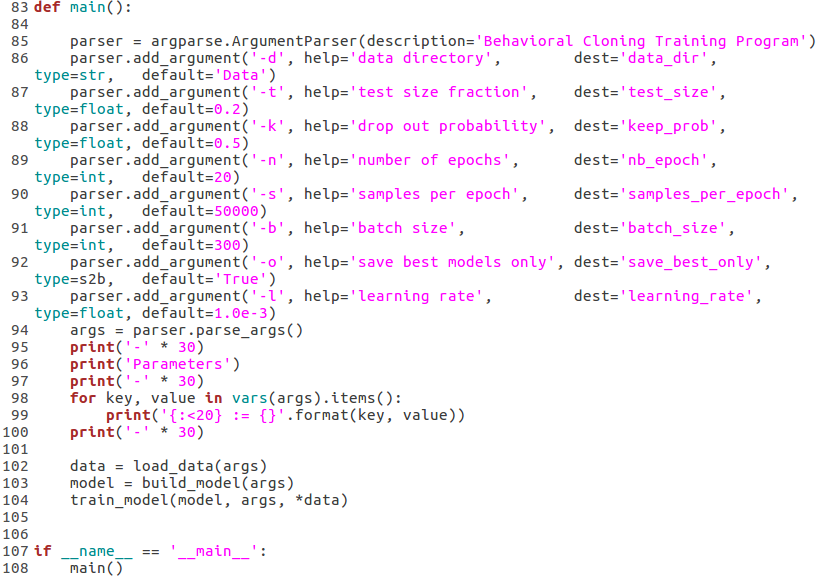
\includegraphics[width=16cm]{fig/15.png}}
		}{
			\Fonte{Elaborado pelo autor}
		}	
\end{figure}

A função inicial do \textit{main()} da Figura\ref{model6}, linha 83,  é a criação de uma instância do \textit{ArgumentParser}, a \textit{parser}, e atribuição dos seus argumentos, da linha 86 a 93.
Após a exibição dos parâmetros na tela, da linha 95 até 100, a função \textit{main()} chama as funções \textit{load\_data(args)}, \textit{build\_lode(args)} e \textit{train\_model(model, args, *data)} com os argumentos criados nessa função.

Ao final, na linha 108, a função \textit{main()} é chamada dentro do loop de verificação para inicar o programa.

\subsection{\textit{utils.py}}
\label{sec:utils.py}

	\begin{figure}[H]
		\centering
		\Caption{\label{utils1}Linhas de código do 1 à 7 arquivo utils.py}
		\UNIFORfig{}{
			\fbox{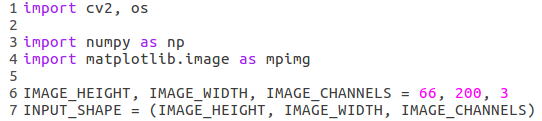
\includegraphics[width=16cm]{fig/16.png}}
		}{
			\Fonte{Elaborado pelo autor}
		}	
\end{figure}
A Figura\ref{utils1} mostra basicamente as bibliotecas que são importadas para esse arquivo( no caso, \textit{OpenCV}, \textit{Miscellaneous operating system interfaces}, \textit{Numpy} e \textit{Matplot}, da linha 1 até a linha 4), atribui valores para as variáveis \textit{IMAGE\_HEIGHT}, \textit{IMAGE\_WIDTH} e \textit{\IMAGE\_CHANNELS} e coloca todas esse valores na tupla \textit{INPUT\_SHAPE}.


\begin{figure}[H]
	\centering
	\Caption{\label{utils2}Linhas de código do 10 à 39 arquivo utils.py}
	\UNIFORfig{}{
		\fbox{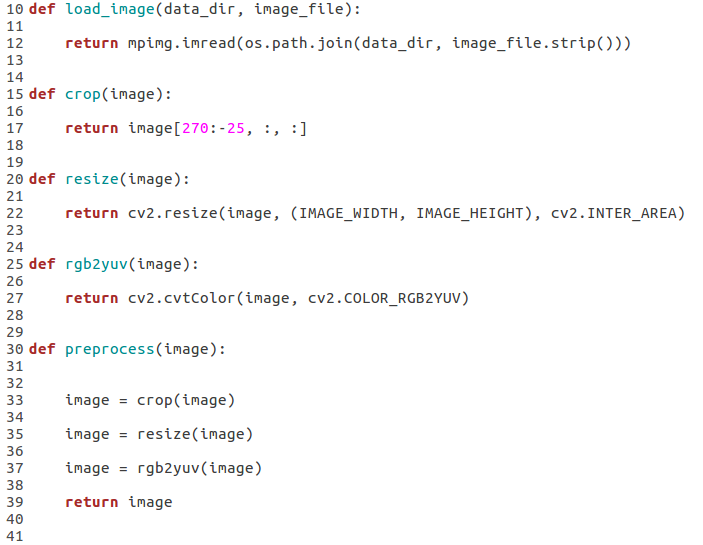
\includegraphics[width=16cm]{fig/17.png}}
	}{
		\Fonte{Elaborado pelo autor}
	}	
\end{figure}

Na Figura\ref{utils2} há cinco métodos, onde o primeiro tem a função de carregar a imagem para o programa (método \textit{load\_image}, linha 10). Os métodos \textit{crop}, \textit{resize} e \textit{rgb2yuv} (na linha 15, 20 e 25, respectivamente) fazem edições nas imagens e o método final, \textit{preprocess(imagem)}, na linha 30, trata de chamar os métodos de edição de imagem.

\begin{figure}[H]
	\centering
	\Caption{\label{utils3}Linhas de código do 42 à 93 arquivo utils.py}
	\UNIFORfig{}{
		\fbox{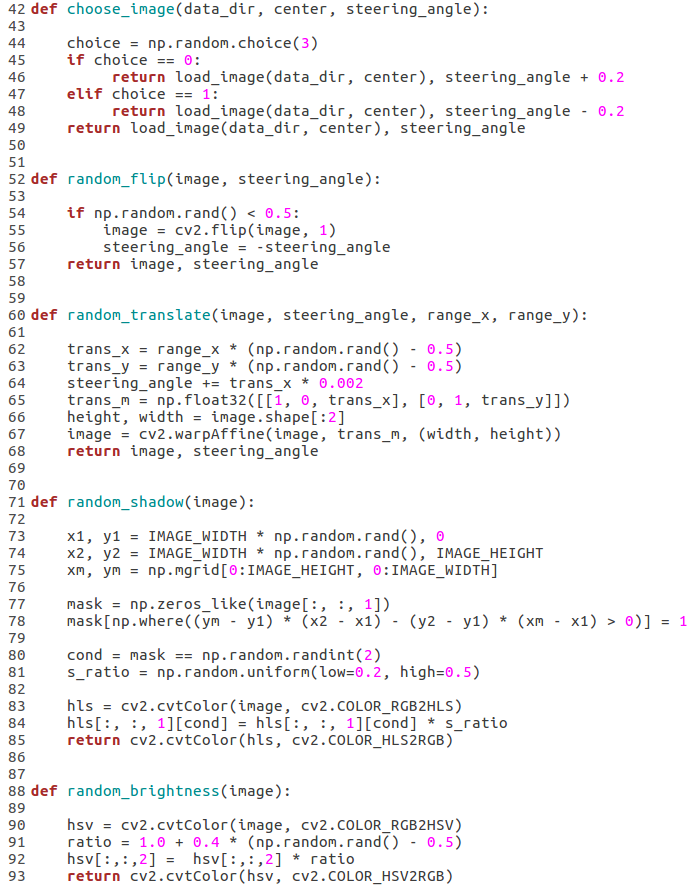
\includegraphics[width=16cm]{fig/18.png}}
	}{
		\Fonte{Elaborado pelo autor}
	}	
\end{figure}

Os métodos utilizados na Figura\ref{utils3} servem para complementar o método \textit{augument()}, modificando a imagem de diversas maneiras.
\begin{description}
    \item[choose\_image(data\_dir, center, steering\_angle):] Linha 42. Escolha aleatoriamente uma imagem e modifica o ângulo de direção.
    \item[random\_flip(image, steering\_angle):] Linha 52. Gira aleatoriamente a imagem para a esquerda ou para a direita, ajustando o ângulo de direção.
    \item[random\_translate(image, steering\_angle, range\_x, range\_y):] Linha 60. Faz uma translação aleatória na imagem.
    \item[random\_shadow(image):] Linha 71. Gera e adiciona sombra aleatória.
    \item[random\_brightness(image):] Linha 88. Ajusta aleatoriamente o brilho da imagem.
\end{description}

\begin{figure}[H]
	\centering
	\Caption{\label{utils4}Linhas de código do 96 à 103 arquivo utils.py}
	\UNIFORfig{}{
		\fbox{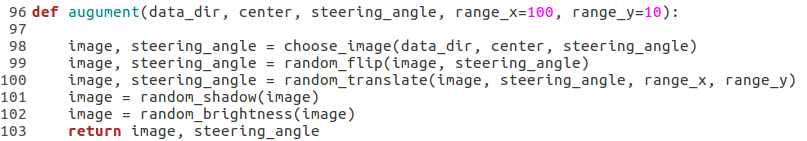
\includegraphics[width=16cm]{fig/19.png}}
	}{
		\Fonte{Elaborado pelo autor}
	}	
\end{figure}

O método \textit{augument()} da linha 96 da Figura\ref{utils4} utiliza os métodos descritos na Figura\ref{utils3}, da linha 42 à 88, para gerar uma imagem diferente das imagens capturadas. Aumentando o número de imagens melhora a previsão da rede neural.

\begin{figure}[H]
	\centering
	\Caption{\label{utils5}Linhas de código do 96 à 103 arquivo utils.py}
	\UNIFORfig{}{
		\fbox{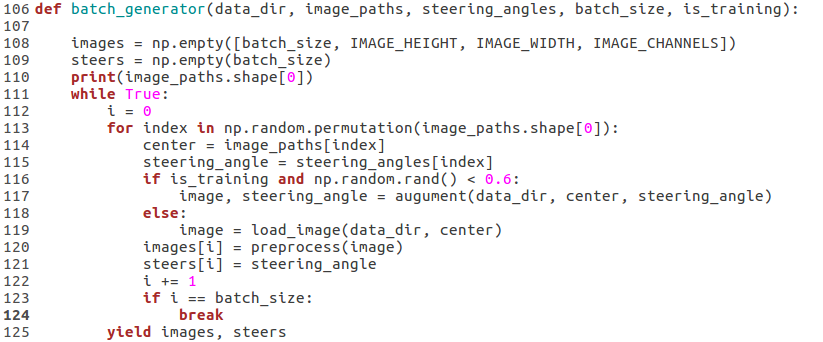
\includegraphics[width=16cm]{fig/20.png}}
	}{
		\Fonte{Elaborado pelo autor}
	}	
\end{figure}

A função \textit{batch\_generator} da Figura\ref{utils5} é gerar imagem de treinamento modificada, fornecer o caminho da imagem e dos ângulos de direção e associar a dois \textit{arrays}: \textit{images} e \textit{steers}. Nesse função é possível escolher se a modificação será feita pelo método \textit{augument()}, citado na Figura\ref{utils4} ou pelo método \textit{preprocess()}, da Figura\ref{utils2}. Para o treinamento da rede neural do projeto, é utilizado o método \textit{augument()} e o método \textit{preprocess()} serve para fazer a validação dos dados treinados.

\subsection{\textit{drive.py}}
\label{sec:drive.py}

\begin{figure}[H]
	\centering
	\Caption{Linhas de código do 1 à 18 arquivo drive.py}
	\UNIFORfig{}{
		\fbox{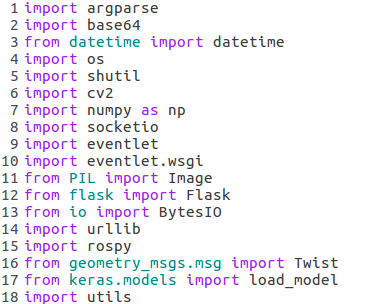
\includegraphics[width=12cm]{fig/6.png}}
	}{
		\Fonte{Elaborado pelo autor}
	}	
\end{figure}

Na linha 1 até a linha 18 do arquivo \textit{drive.py} são importadas as bibliotecas essenciais para o funcionamento do programa.

\begin{figure}[H]
	\centering
	\Caption{{\label{figura 7}}Linhas de código do 20 à 29 arquivo drive.py}
	\UNIFORfig{}{
		\fbox{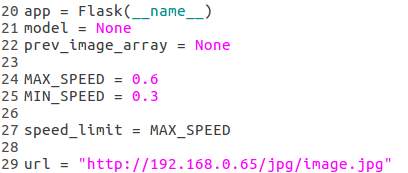
\includegraphics[width=12cm]{fig/7.png}}
	}{
		\Fonte{Elaborado pelo autor}
	}	
\end{figure}

Na Figura\ref{figura 7}, da linha 20 até á 25, são declaradas as variáveis a serem utilizadas no restante do programa. Na linha 27 a velocidade máxima é limitada ao valor de \textit{MAX\_SPEED} e na linha 29 o link da câmera IP é atribuído à variável \textit{url}.
\begin{figure}[H]
	\centering
	\Caption{{\label{figura 8}}Linhas de código do 20 à 29 arquivo drive.py}
	\UNIFORfig{}{
		\fbox{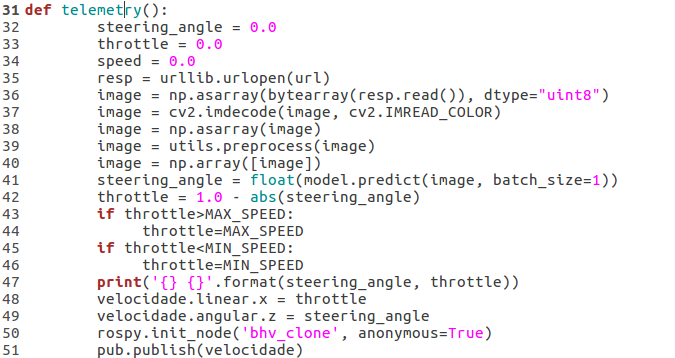
\includegraphics[width=14cm]{fig/8.png}}
	}{
		\Fonte{Elaborado pelo autor}
	}	
\end{figure}

Na linha 31, a função \textit{telemetry()} da Figura\ref{figura 8} começa zerando os valores das variáveis \textit{steering\_angle, throttle} e \textit{speed}. Na linha 35 ele recebe a imagem capturada pelo Jaguar e faz a tratamento dela com os mesmos valores utilizados para criar o modelo. Na linha 41 é criado a previsão para a imagem analisada e salva na instância \textit{steering\_angle}. O \textit{throttle} recebe o valor de 1 menos o módulo do ângulo de direção para diminuir a velocidade conforme ele gira. As linhas 43 e 45 garantem que o valor de velocidade seja sempre menor que valor máximo.

Ao final da função \textit{telemetry()} os valores de \textit{steering\_angle} e \textit{throttle} são imprimidos na tela e colocados nas variáveis \textit{velocidade.linear.x} e \textit{velocidade.angular.z} para finalmente serem publicados no  \textit{Node} do Jaguar.

\begin{figure}[H]
	\centering
	\Caption{{\label{figura 9}}Linhas de código do 53 à 74 arquivo drive.py}
	\UNIFORfig{}{
		\fbox{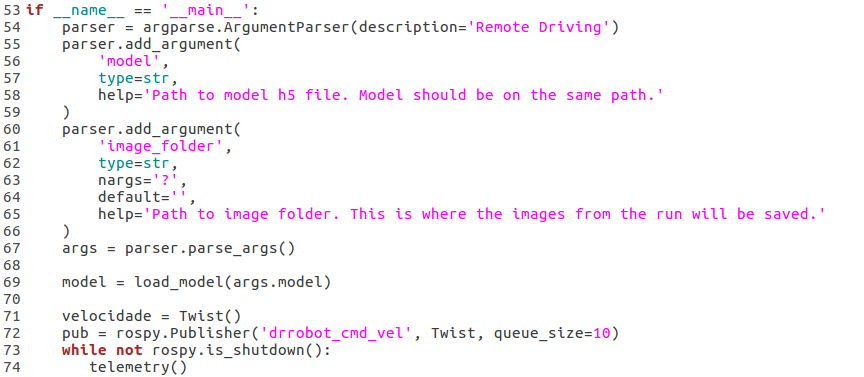
\includegraphics[width=16cm]{fig/9.png}}
	}{
		\Fonte{Elaborado pelo autor}
	}	
\end{figure}

Dentro da função \textit{main()}, da linha 54 até a linha 67, são criados os argumentos de localização do modelo e da pasta de imagens. Essa localização tem que ser fornecida pelo usuário no momento de execução do programa. A instância velocidade recebe então a função \textit{Twist()} e é criado, na linha 72, um tópico chamado \textit{pup} para a publicação de mensagens no \textit{Node} do Jaguar. Na linha 73, enquanto o \textit{Node} do \textit{Jaguar} estiver ligado a função \textit{main()} irá continuar chamando a função \textit{telemetry()}.